
\subsection{MiniCPM-DPO}
\label{app:rlhf}
After SFT, we employ DPO~\citep{rafailov2024direct} for human preference alignment of the
model. During this stage, UltraFeedback~\citep{cui2023ultrafeedback} is utilized as the primary alignment dataset, and a proprietary preference dataset is constructed to enhance the model's code and mathematical capabilities. We conduct one epoch of DPO training with a learning rate of $1\times 10^{-5}$ and utilize a Cosine LRS since we have a pre-defined training step.
 
After applying DPO for preference alignment, the model's score on MTBench~\citep{zheng2024judging} increased from 6.89 after SFT to 7.25, surpassing even large models such as Llama2-70B-Chat (see Figure~\ref{fig:mtbenchscore}). However, we also noticed that the performance on benchmarks is slightly compromised, which is known as the alignment tax~\citep{askell2021general}.

\begin{table}[htbp]
    \centering
\scalebox{0.87}{

\begin{tabular}{lccccccccc}
\toprule
\textbf{Model} & \textbf{C-Eval} & \textbf{CMMLU} & \textbf{MMLU} & \textbf{HumanEval} & \textbf{MBPP} & \textbf{GSM8K} & \textbf{MATH}\\
\midrule
ChatGLM2-6B & 52.05 & 49.21 & 45.77 & 10.37 & 9.38 & 22.74 & 5.96 \\
Mistral-7B-Instruct-v0.1 & 38.06 & 36.96 & 53.56 & 29.27 & 39.34 & 28.73 & 3.48\\
Mistral-7B-Instruct-v0.2 & 42.55 & 41.92 & 60.51 & 36.59 & 48.95 & 40.49 & 4.95 \\
Qwen-7B-Chat & 58.57 & 57.23 & 56.03 & 15.85 & 40.52 & 42.23 & 8.3\\
Yi-6B-Chat & 70.88 & 71.11 & 62.95 & 14.02 & 28.34 & 36.54 & 3.88\\
Baichuan2-7B-Chat & 53.28 & 53.50 & 53.00 & 21.34 & 32.32 & 25.25 & 6.32\\
Deepseek-7B-chat & 46.95 & 49.72 & 51.67 & 40.85 & 48.48 & 48.52 & 4.26 \\
Llama2-7B-Chat & 34.54 & 32.64 & 47.64 & 14.02 & 27.40 & 21.15 & 2.08 \\
\midrule
\textbf{MiniCPM-2.4B-DPO}  & 48.64 & 48.37 & 53.05 & 51.22 & 48.01 & 53.37 & 9.86\\
\bottomrule
\end{tabular}
}

\scalebox{0.88}{
\begin{tabular}{lccccccc}
\toprule
\textbf{Model}  & \textbf{BBH} &\textbf{ ARC-e} & \textbf{ARC-c} & \textbf{HellaSwag} & \textbf{Avg} & \textbf{Avg$_{\text{en}}$} & \textbf{Avg$_{\text{chn}}$}  \\
\midrule
ChatGLM2-6B  & 32.60 & 74.45 & 56.82 & 58.48$^{\dag}$ & 37.98 & 35.17 & 50.63 \\
Mistral-7B-Instruct-v0.1  & 39.52 & 81.61 & 63.99 & 73.47$^{\dag}$ & 44.36 & 45.89 & 37.51 \\
Mistral-7B-Instruct-v0.2  & 39.81 & 86.28 & 73.38 & 84.55$^{\dag}$ & 50.91 & 52.83 & 42.24 \\
Qwen-7B-Chat  & 37.34 & 64.44$^{\dag}$ & 39.25$^{\dag}$ & 74.52$^{\dag}$ & 44.93 & 42.05 & 57.90 \\
Yi-6B-Chat  & 37.43 & 84.89 & 70.39 & 74.60$^{\dag}$ & 50.46 & 45.89 & 71.00 \\
Baichuan2-7B-Chat  & 37.46 & 79.63 & 60.15 & 69.23$^{\dag}$ & 44.68 & 42.74 & 53.39 \\
Deepseek-7B-chat  & 35.70 & 76.85 & 63.05 & 76.68$^{\dag}$ & 49.34 & 49.56 & 48.34 \\
Llama2-7B-Chat  & 35.54 & 74.28 & 54.78 & 75.65$^{\dag}$ & 38.16 & 39.17 & 33.59 \\
\midrule
\textbf{MiniCPM-2.4B-DPO}  & 36.22 & 85.02 & 68.17 & 65.67 & 51.60 & 52.29 & 48.51 \\
\bottomrule
\end{tabular}
}
\caption{Benchmark scores for MiniCPM-2.4B-DPO compared with larger chat models.}
\label{tab:benchmark}
\end{table}


\begin{figure}
    \centering
    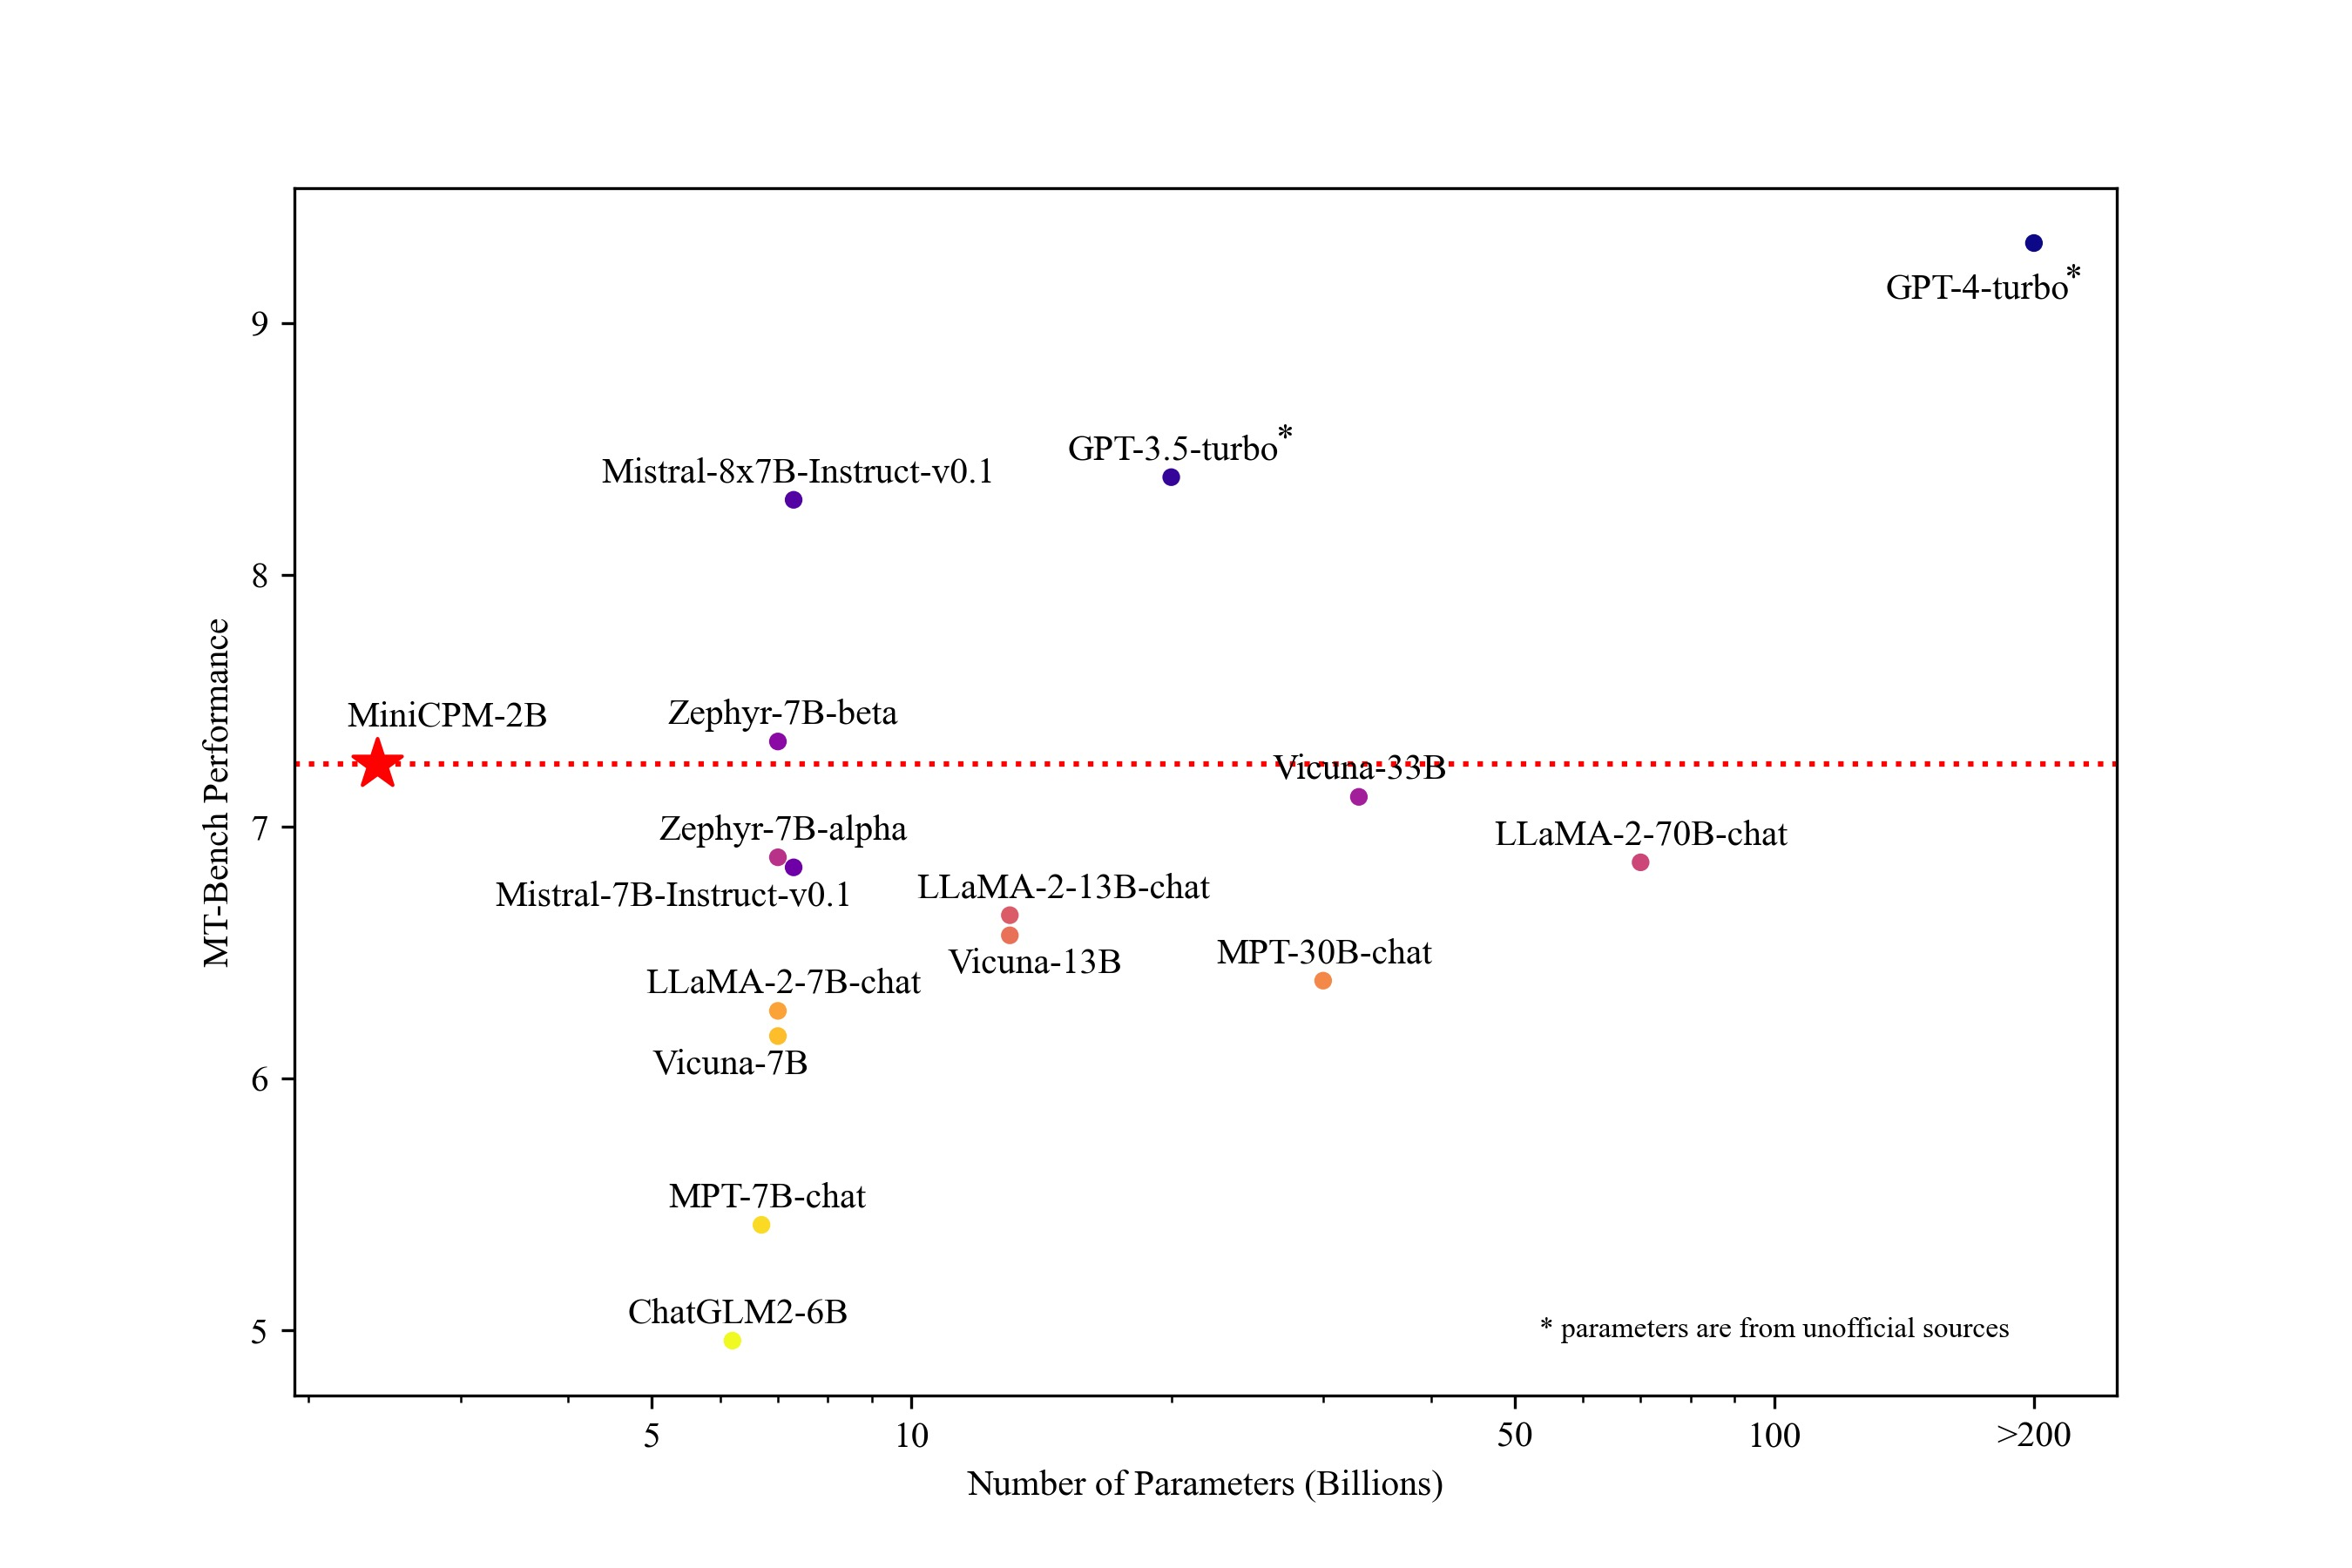
\includegraphics[width=0.7\linewidth]{Fig/mtbench_graph.jpg}
    \caption{MTBench score of MiniCPM-DPO-2.4B surpasses many models of larger size. }
    \label{fig:mtbenchscore}
    \vspace{-5mm}
\end{figure}


